% -----------------------------------------------------------------------------
% UFRJ
% PPGI
% MAB 733 Sistemas Distribuídos
%
% Revisado em <não revisado>
% Aluno: Cristiano Gurgel de Castro
% -----------------------------------------------------------------------------

\chapter{Desenvolvimento e Arquitetura}

O programa é composto por uma aplicação desktop cliente Java. Essa aplicação
simples trata-se de uma calculadora que efetua as quatro operações básicas.
A camada de negócio da calculadora simples trata portanto dessas 4 operações básicas:
\texttt{add}, \texttt{subtract}, \texttt{multiply}, \texttt{divide}.

No projeto da calculadora foi criada uma fachada para essa camada de negócios:
\texttt{IMathOperations} e duas implementações desta fachada:
\texttt{MathOperations}, que é local, e \texttt{RemoteMathOperations}. Esta
última utiliza contém os métodos para utilização de um \WebService.


\begin{figure}[htb]
  \centering
  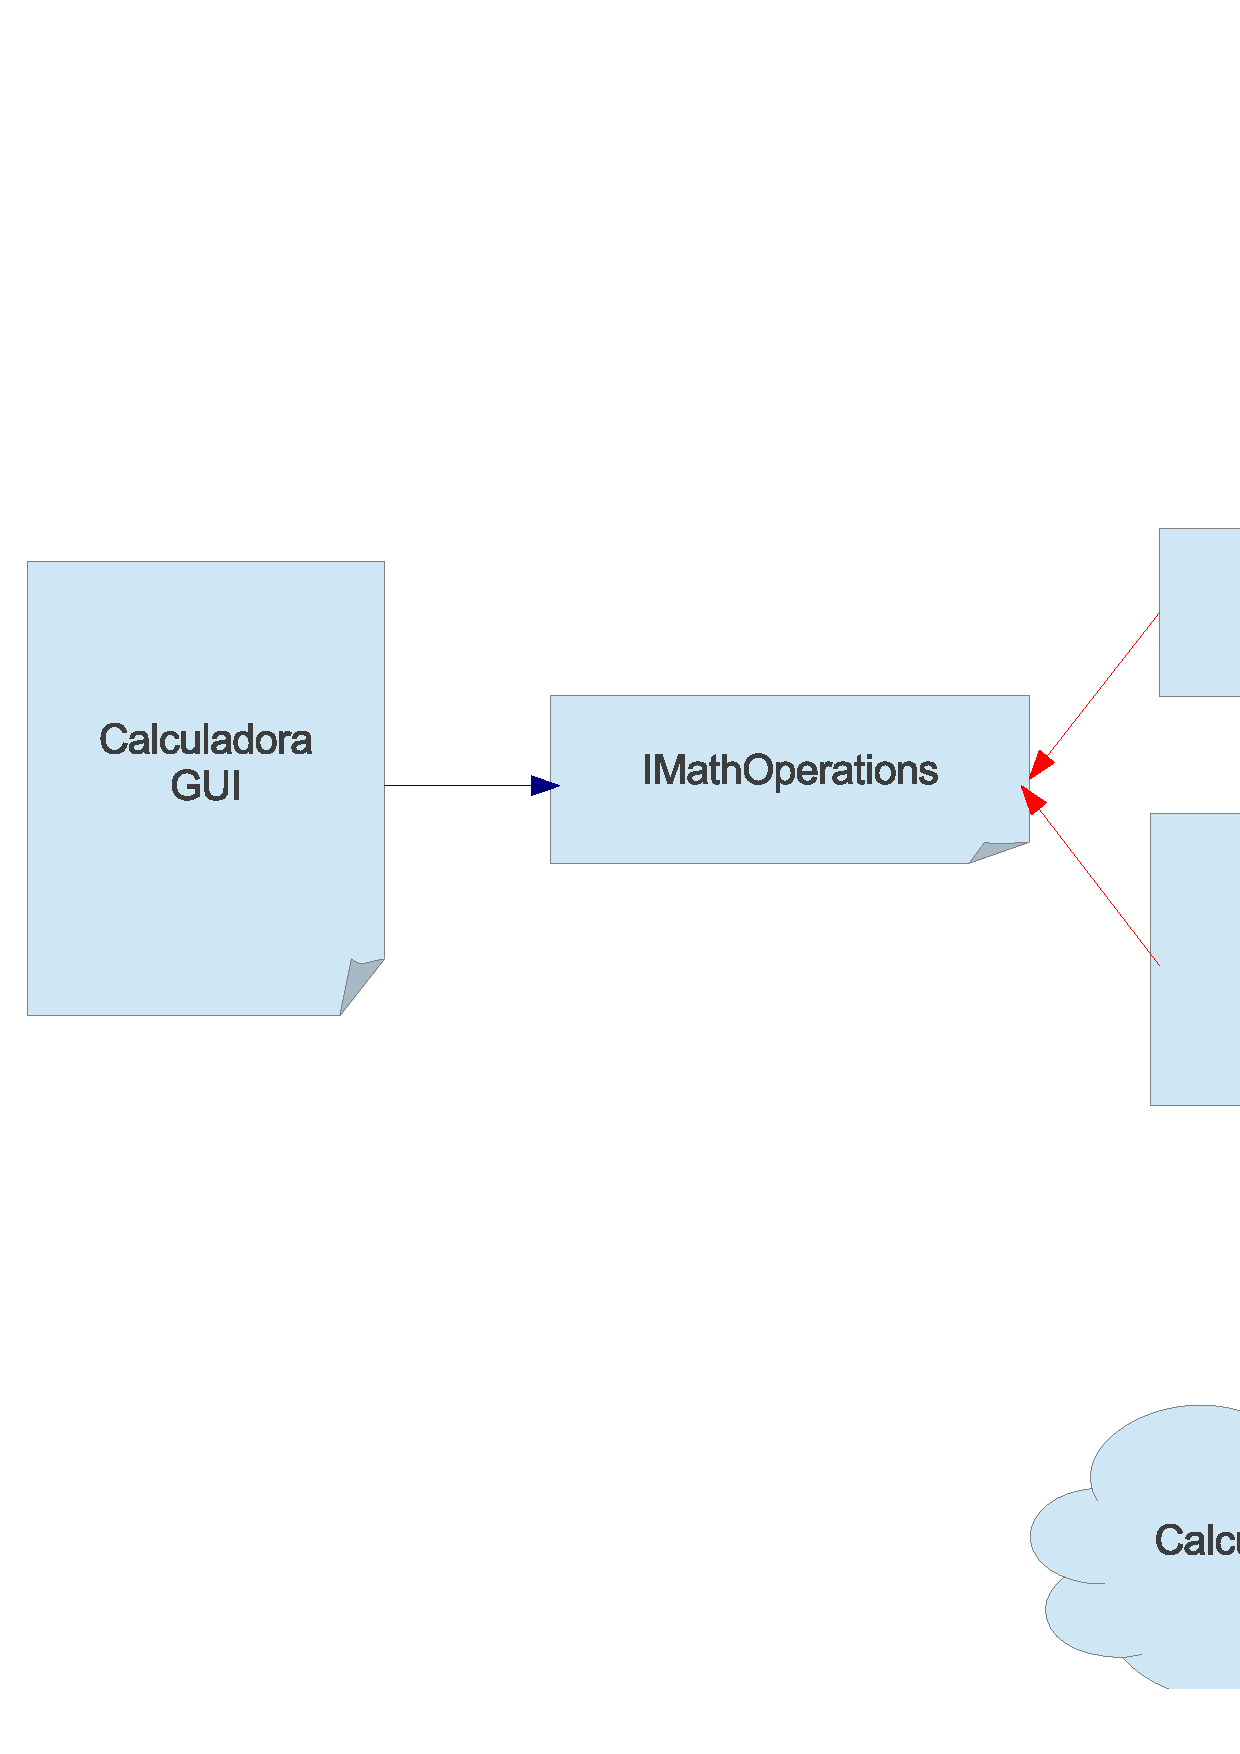
\includegraphics[width=0.5\textwidth]{imgs/calculadora}
  \caption{Arquitetura da aplicação cliente. As setas azuis representam a
    relação \textit{Utiliza}, já as setas vermelhas representam a relação
  \textit{Implementa}}.
  \label{fig:arquitetura:calc}
\end{figure}

Um trecho do código da classe \texttt{RemoteMathOperations} com a chamada ao
método de soma do serviço Web é mostrado no Código \ref{cod:add}.

\begin{lstlisting}[float,caption=Operação de chamada ao WebService,label=cod:add,language=Java]
private static float add(float i, float j) {
  org.me.calculator.CalculatorWS_Service service = 
    new org.me.calculator.CalculatorWS_Service();
  org.me.calculator.CalculatorWS port = 
    service.getCalculatorWSPort();
  return port.add(i, j);
}
\end{lstlisting}

% TODO colocar um delimitador antes e depois dos códigos

O serviço \texttt{CalculatorWebService} provê uma implementação das quatro
operações básicas utilizadas pela calculadora. O \WebService\ foi criado utilizando o IDE
\NetBeans\ juntamente com seu servidor de aplicação \Glassfish, no qual foi hospedado o
serviço. O \NetBeans\ provê uma funcionalidade muito prática de criação de
\WebService s, através da utilização da opção ``Serviço Web'' do Assistente de criação de
projetos. O \NetBeans\ automaticamente cria uma classe com a implementação do
Serviço Web. O usuário pode visualizar uma tela chamada 
``Design'' contendo uma visualização amigável das operações efetuadas a serem
implementadas no serviço (ver Figura \ref{fig:arquitetura:design}). Através
dessa tela, foram configuradas as quatro operações que o \WebService\ deve
fornecer: as quatro operações básicas. Cada uma dessas operações recebem dois
\texttt{float}s como parâmetros e retornam um \texttt{float} como resultado.
Após as configurações configurações das operações, a tarefa seguinte foi inserir
o código de implementação. Um trecho de código exemplo, com a operação de adição
do \WebService, é mostrado abaixo no código \ref{cod:calculatorws}:

\lstinputlisting[caption=Serviço de calculadora,label=cod:calculatorws,firstline=14,lastline=25]{codes/CalculatorWS.java}

\begin{figure}[htb]
  \centering
  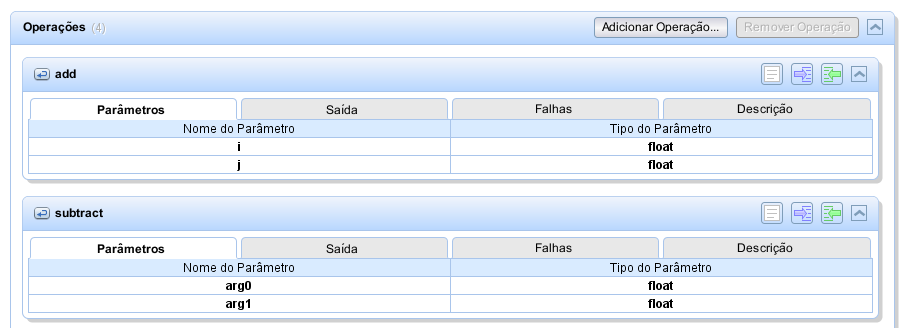
\includegraphics[width=\textwidth]{imgs/webservice-design}
  \caption{Tela de design de um \WebService}
  \label{fig:arquitetura:design}
\end{figure}

Foi utilizado a linguagem de programação PHP para a criação de um outro serviço
local com a implementação das operações de soma, subtração, multiplicação e
divisão. Para o teste desse servidor foi criado cliente também PHP. Notou-se que
a configuração de uma relação cliente servidor em PHP pode ser feita sem maiores
dificuldades.

Dois serviços externos foram considerados. Um deles foi o \textit{Number
Converter} encontrado a partir do site \url{xmethods.net}. Segundo sua descrição
ele possui dois métodos: o primeiro contém um serviço de escrita por extenso na
língua inglesa, recebendo como parâmetro um inteiro, o segundo contém uma
funcionalidade semelhante para conversão para valores monetários em dólar.

Para o acesso ao serviço Web foi utilizada uma facilidade do \NetBeans\ na
aplicação cliente da calculadora: a criação de um ``Cliente para serviço Web''.
Esse componente da IDE foi adicionada ao projeto cliente de calculadora, e
através de um Assistente para a configuração, foi informada a URL do WSDL do
serviço, a saber
\url{http://www.dataaccess.com/webservicesserver/numberconversion.wso?WSDL} Uma
funcionalidade ``SAY'' foi adicionada ao projeto para a chamada ao serviço. Uma
classe \texttt{NumberToWords} foi criada para a executar a chamada ao
\WebService. A chamada ao serviço web externo é mostrado no código
\ref{cod:numberconv}.

\lstinputlisting[float,caption=Chamada ao serviço web
externo, label=cod:numberconv,firstline=22,lastline=28]{codes/NumberToWords.java}

No entanto um erro de transporte HTTP, foi lançado durante a chamada de serviço:

\begin{lstlisting}
Exception in thread "AWT-EventQueue-0" 
com.sun.xml.internal.ws.client.ClientTransportException: 
HTTP transport error: java.net.ConnectException: 
Connection timed out: connect
\end{lstlisting}

Interessante notar que um outro projeto cliente Java foi criado para testar a
comunicação com o serviço Web \texttt{numberconversion} e a comunicação ocorreu
sem maiores problemas.  Um outro cliente, escrito na linguagem \php\ também
executou normalmente o acesso ao serviço. O Código \ref{cod:phpclient} mostra o
acesso ao serviço externo com um cliente \php. 

\lstinputlisting[label=cod:phpclient,language=php]{codes/NumberConversion.php}.

Foi criado também outro cliente \php\ para consumir um serviço externo de
conversão de temperatura, através da URL
\url{http://www.webservicex.net/ConvertTemperature.asmx?WSDL} no entanto, nos
deparamos com uma falha no próprio serviço executado:

\begin{lstlisting}
System.IO.IOException: There is not enough space on the disk.
\end{lstlisting}

